\section{Altri Risultati}\label{sec:altri-risultati}
\subsection{Mean-field approximation}\label{subsec:app-mean-field-approximation}
    \begin{figure}[H]
        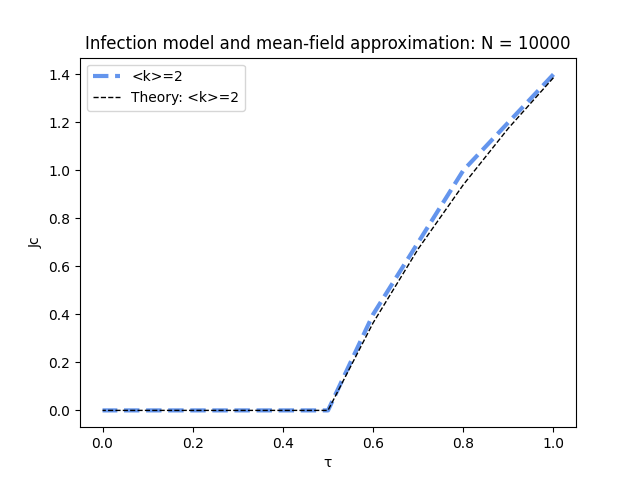
\includegraphics[width=\textwidth]{MF/k2-it10000}\caption{Mean-field approximation with $k=2$}
        \label{fig:mf_k_2}
    \end{figure}
    \begin{figure}[H]
        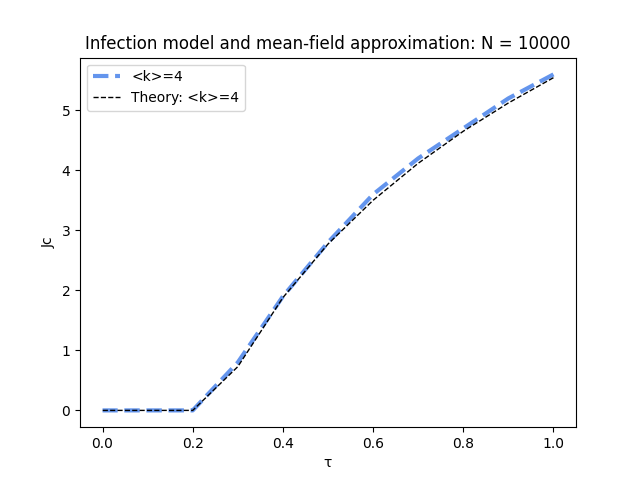
\includegraphics[width=\textwidth]{MF/k4-it10000}\caption{Mean-field approximation with $k=4$}
        \label{fig:mf_k_4}
    \end{figure}
    \begin{figure}[H]
        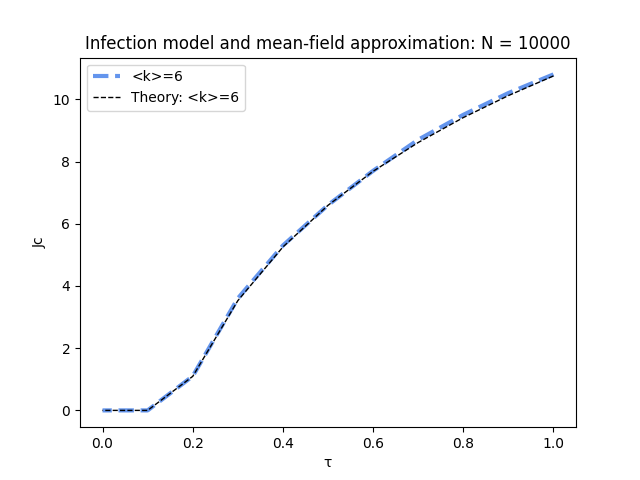
\includegraphics[width=\textwidth]{MF/k6-it10000}\caption{Mean-field approximation with $k=6$}
        \label{fig:mf_k_6}
    \end{figure}

\subsection{Simple percolation}\label{subsec:app-simple-percolation}
    \begin{figure}[H]
        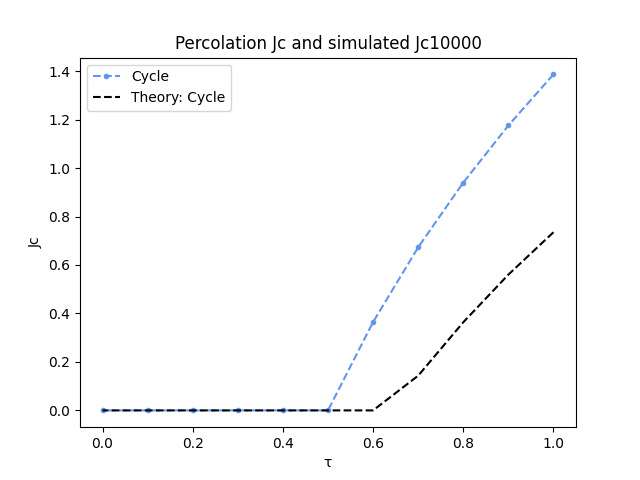
\includegraphics[width=\linewidth]{/C:/Users/loreb/Documents/IntellijProjects/PycharmProjects/Epydemic/results/plots/SIM/Cycle-nodes10000_it10000}\caption{Simple percolation Cycle with $k=2$}
        \label{fig:sim_cycle}
    \end{figure}
    \begin{figure}[H]
        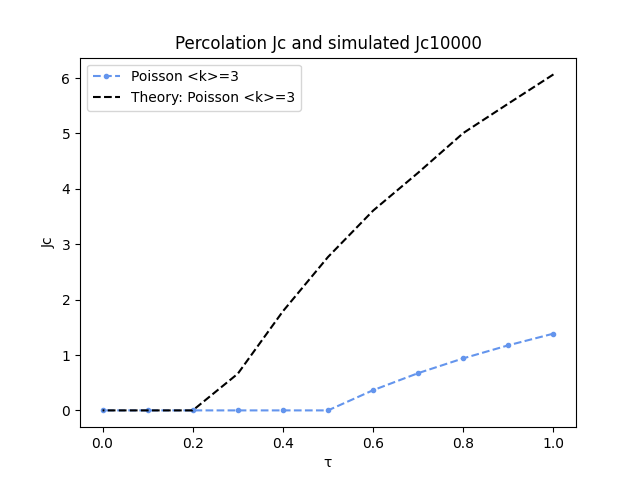
\includegraphics[width=\linewidth]{/C:/Users/loreb/Documents/IntellijProjects/PycharmProjects/Epydemic/results/plots/SIM/Poisson-k3_nodes10000_it10000}\caption{Simple percolation Poisson with $k=3$}
        \label{fig:sim_poisson_k_3}
    \end{figure}
    \begin{figure}[H]
        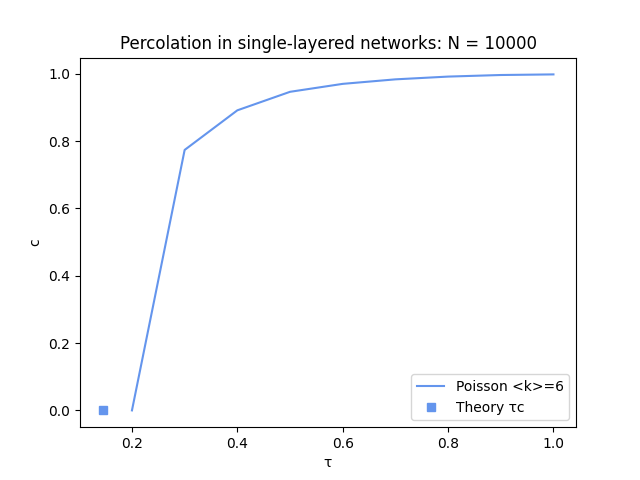
\includegraphics[width=\linewidth]{/C:/Users/loreb/Documents/IntellijProjects/PycharmProjects/Epydemic/results/plots/SIM/Poisson-k6_nodes10000_it10000}\caption{Simple percolation Poisson with $k=6$}
        \label{fig:sim_poisson_k_6}
    \end{figure}
    \begin{figure}[H]
        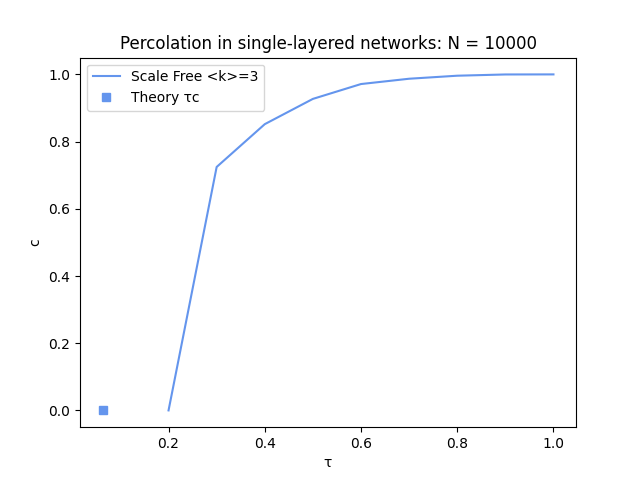
\includegraphics[width=\linewidth]{/C:/Users/loreb/Documents/IntellijProjects/PycharmProjects/Epydemic/results/plots/SIM/ScaleFree-k3_nodes10000_it10000}\caption{Simple percolation Scale-Free with $k=3$}
        \label{fig:sim_scale_free_k_3}
    \end{figure}

\subsection{Infezione percezione del rischio}\label{subsec:app-infezione-con-la-percezione-del-rischio}
    \begin{figure}[H]
        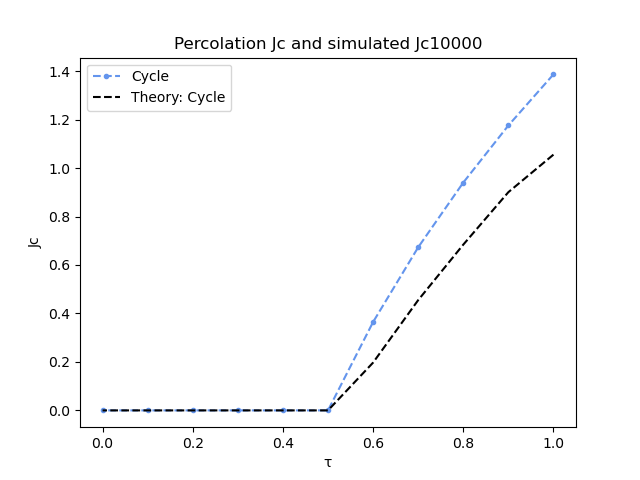
\includegraphics[width=\textwidth]{/C:/Users/loreb/Documents/IntellijProjects/PycharmProjects/Epydemic/results/plots/PERC/Cycle-nodes10000_it100}\caption{Self percolation Cycle with $k=2$}
        \label{fig:perc_cycle}
    \end{figure}
    \begin{figure}[H]
        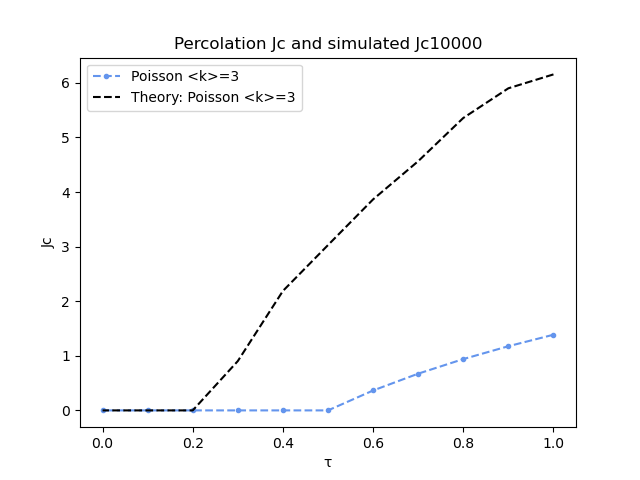
\includegraphics[width=\textwidth]{/C:/Users/loreb/Documents/IntellijProjects/PycharmProjects/Epydemic/results/plots/PERC/Poisson-k3_nodes10000_it100}\caption{Self percolation Poisson with $k=3$}
        \label{fig:perc_poisson_k_3}
    \end{figure}
    \begin{figure}[H]
        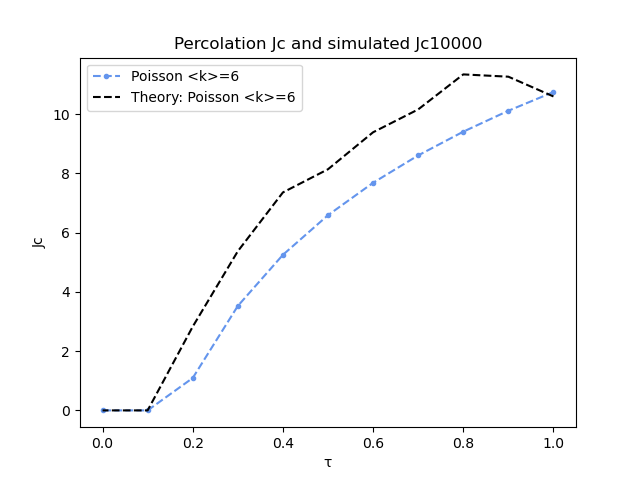
\includegraphics[width=\textwidth]{/C:/Users/loreb/Documents/IntellijProjects/PycharmProjects/Epydemic/results/plots/PERC/Poisson-k6_nodes10000_it100}\caption{Self percolation Poisson with $k=6$}
        \label{fig:perc_poisson_k_6}
    \end{figure}
    \begin{figure}[H]
        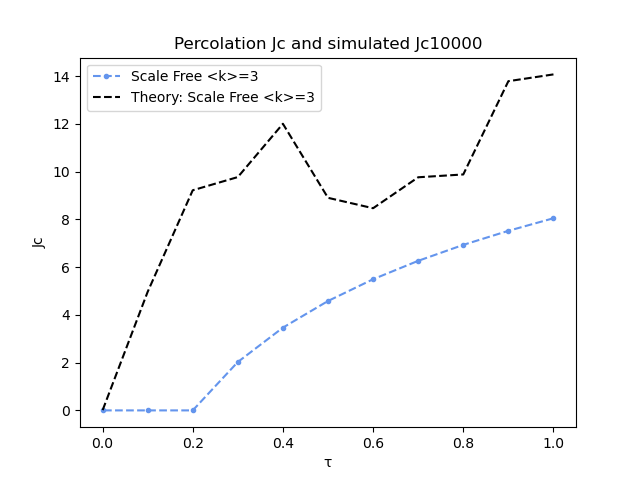
\includegraphics[width=\textwidth]{/C:/Users/loreb/Documents/IntellijProjects/PycharmProjects/Epydemic/results/plots/PERC/ScaleFree-k3_nodes10000_it100}\caption{Self percolation Scale-Free with $k=3$}
        \label{fig:perc_scale_free_k_3}
    \end{figure}
    \begin{figure}[H]
        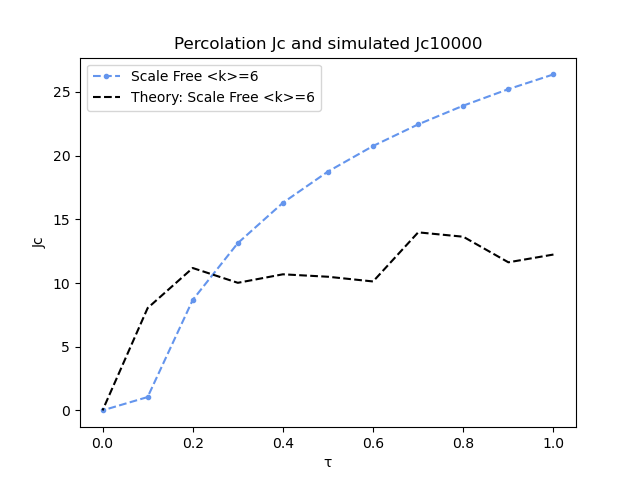
\includegraphics[width=\textwidth]{/C:/Users/loreb/Documents/IntellijProjects/PycharmProjects/Epydemic/results/plots/PERC/ScaleFree-k6_nodes10000_it100}\caption{Self percolation Scale-Free with $k=6$}
        \label{fig:perc_scale_free_k_6}
    \end{figure}

\subsection{Multiplex networks}\label{subsec:app-multiplex-networks}
    \begin{figure}[H]
        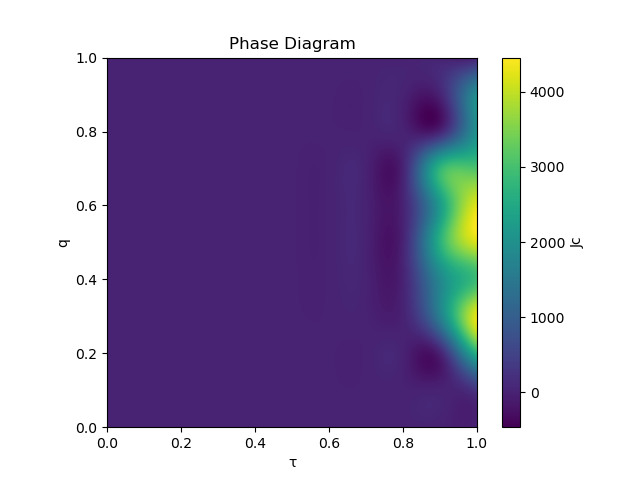
\includegraphics[width=\textwidth]{/C:/Users/loreb/Documents/IntellijProjects/PycharmProjects/Epydemic/results/plots/MUL/Cycle-nodes10000_it100_jminf}\caption{Multiplex Cycle with $k=2$}
        \label{fig:multi_cycle}
    \end{figure}
    \begin{figure}[H]
        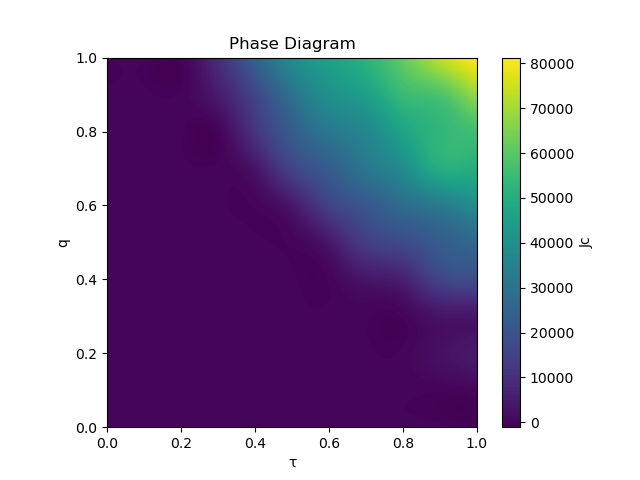
\includegraphics[width=\textwidth]{/C:/Users/loreb/Documents/IntellijProjects/PycharmProjects/Epydemic/results/plots/MUL/Poisson-k3_nodes10000_it100_jminf}\caption{Multiplex Poisson with $k=3$}
        \label{fig:multi_poisson_k_3}
    \end{figure}
    \begin{figure}[H]
        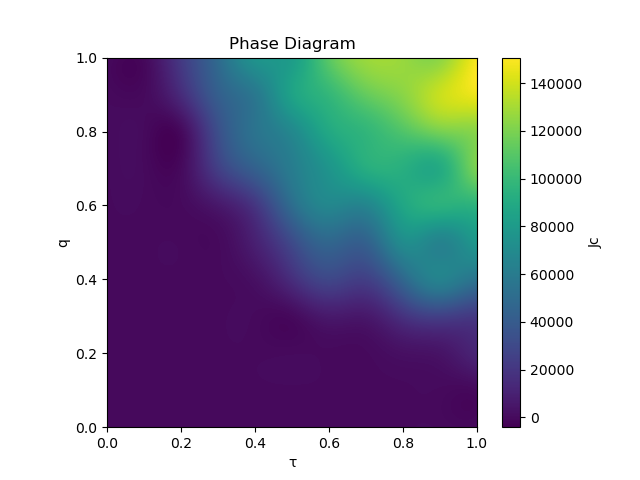
\includegraphics[width=\textwidth]{/C:/Users/loreb/Documents/IntellijProjects/PycharmProjects/Epydemic/results/plots/MUL/Poisson-k6_nodes10000_it100_jminf}\caption{Multiplex Poisson with $k=6$}
        \label{fig:multi_poisson_k_6}
    \end{figure}
    \begin{figure}[H]
        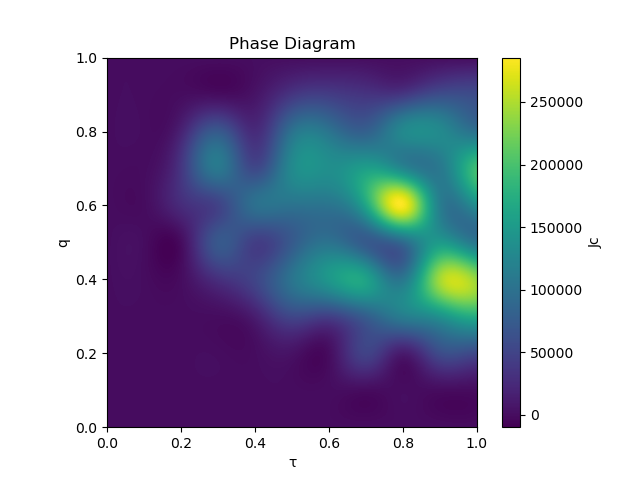
\includegraphics[width=\textwidth]{/C:/Users/loreb/Documents/IntellijProjects/PycharmProjects/Epydemic/results/plots/MUL/ScaleFree-k3_nodes10000_it100_jminf}\caption{Multiplex Scale-Free with $k=3$}
        \label{fig:multi_scale_free_k_3}
    \end{figure}
    \begin{figure}[H]
        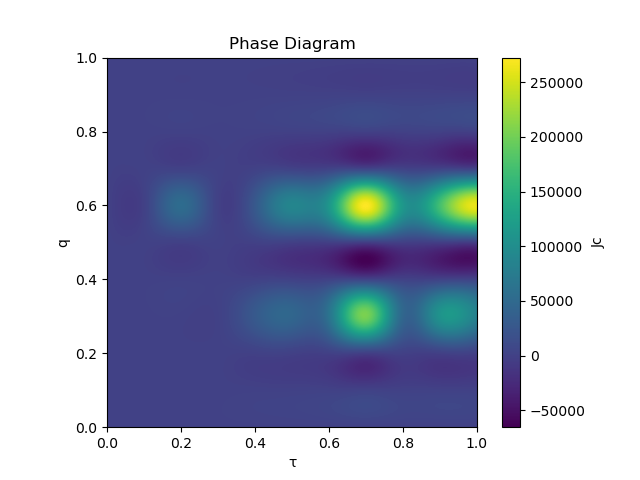
\includegraphics[width=\textwidth]{/C:/Users/loreb/Documents/IntellijProjects/PycharmProjects/Epydemic/results/plots/MUL/ScaleFree-k6_nodes10000_it100_jminf}\caption{Multiplex Scale-Free with $k=6$}
        \label{fig:multi_scale_free_k_6}
    \end{figure}
    \begin{figure}[H]
        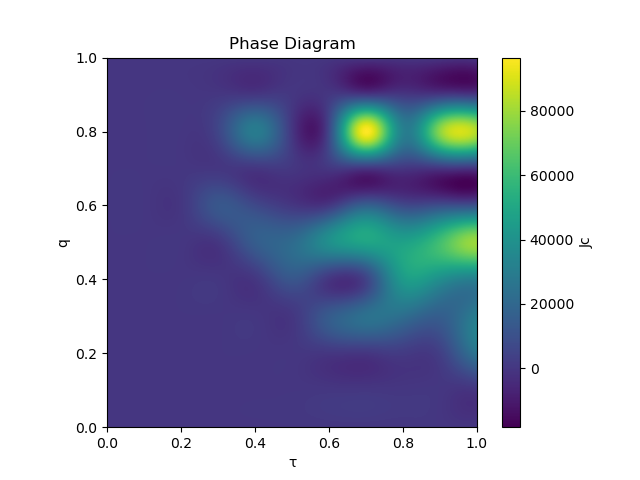
\includegraphics[width=\textwidth]{/C:/Users/loreb/Documents/IntellijProjects/PycharmProjects/Epydemic/results/plots/MUL/Poisson-k6+ScaleFree-k6_nodes10000_it100_jminf}\caption{Multiplex Poisson with $k=6$}
        \label{fig:multi_poisson_k_6_5}
    \end{figure}

    \subsubsection{Limite a Jc = 100}
    \begin{figure}[H]
        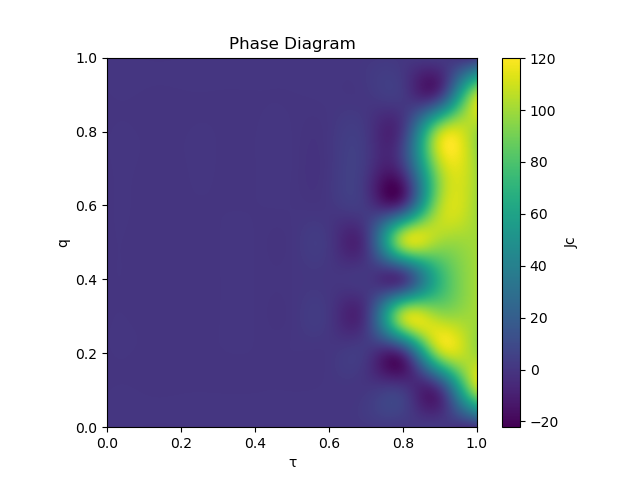
\includegraphics[width=\textwidth]{/C:/Users/loreb/Documents/IntellijProjects/PycharmProjects/Epydemic/results/plots/MUL/Cycle-nodes10000_it100_jm100}\caption{Multiplex Poisson with $k=6$}
        \label{fig:multi_poisson_k_6_2}
    \end{figure}
    \begin{figure}[H]
        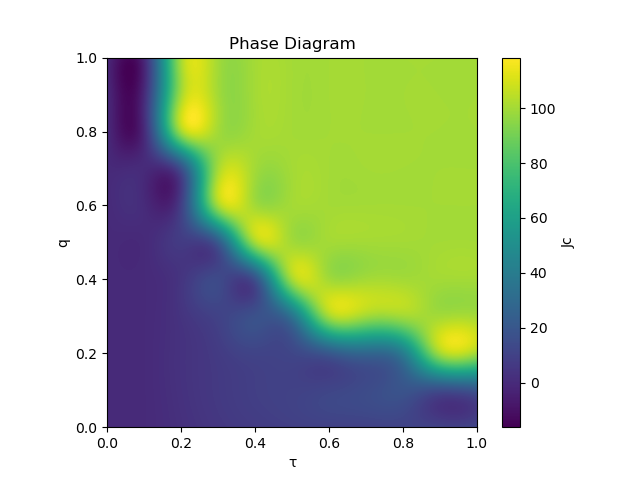
\includegraphics[width=\textwidth]{/C:/Users/loreb/Documents/IntellijProjects/PycharmProjects/Epydemic/results/plots/MUL/Poisson-k6_nodes10000_it100_jm100}\caption{Multiplex Poisson with $k=6$}
        \label{fig:multi_poisson_k_6_3}
    \end{figure}
    \begin{figure}[H]
        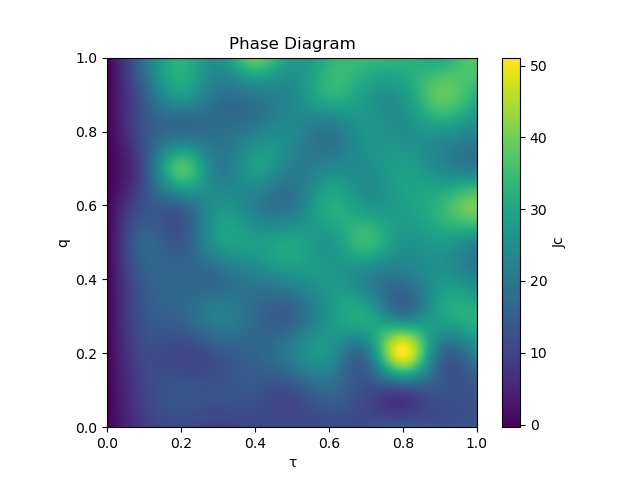
\includegraphics[width=\textwidth]{/C:/Users/loreb/Documents/IntellijProjects/PycharmProjects/Epydemic/results/plots/MUL/ScaleFree-k6_nodes10000_it100_jm100}\caption{Multiplex Poisson with $k=6$}
        \label{fig:multi_poisson_k_6_4}
    \end{figure}
    \begin{figure}[H]
        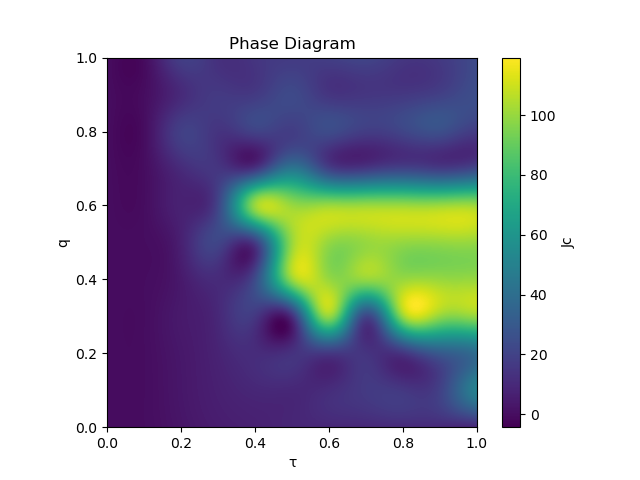
\includegraphics[width=\textwidth]{/C:/Users/loreb/Documents/IntellijProjects/PycharmProjects/Epydemic/results/plots/MUL/Poisson-k6+ScaleFree-k6_nodes_10000_it100_jm100}\caption{Multiplex Poisson with $k=3$}
        \label{fig:multi_poisson_k_3_2}
    \end{figure}
